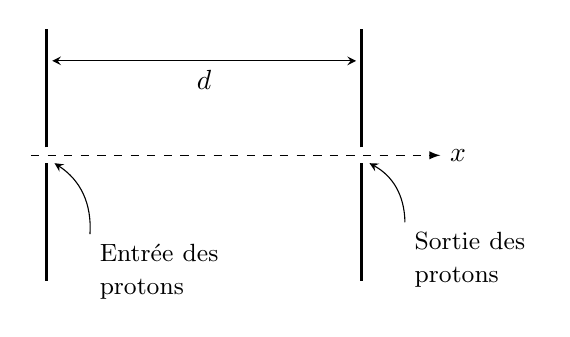
\begin{tikzpicture}
%\draw (-1.75,-0.45) rectangle (-0.2,0.45) node[midway,text centered, text width=1.5cm]{\footnotesize{Source de protons}};
\draw[-latex,dashed] (-0.2,0) -- (5,0) node[right]{$x$};
\draw[very thick] (0,-0.1) -- +(0,-1.5);
\draw[very thick] (0,0.1) -- +(0,1.5) ;
\draw[very thick] (4,-0.1) -- +(0,-1.5);
\draw[very thick] (4,0.1) -- +(0,1.5) ;
%\draw (0,0) node[above right]{$O$};
\draw (0,0) node[above left]{$\ptO$};
\draw (4,0) node[above right]{$\ptS$};
\draw[stealth-stealth,shorten <=2pt,shorten >=2pt] (0,1.2) -- +(4,0) node[midway,below]{$d$};
\draw[stealth-] (0.1,-0.1) to[bend left] +(0.45,-0.9) node[below right,text width=2cm]{\small Entrée des protons};
\draw[stealth-] (4.1,-0.1) to[bend left] +(0.45,-0.75) node[below right,text width=1.5cm]{\small Sortie des protons};
\end{tikzpicture}